\section{Relação: Algoritmos x Programas}

\begin{frame}{Sobre o computador}
  O que é um computador?
  \pause
  \begin{itemize}
    \item Uma máquina abstrata com uma fita (memória) infinita e um conjunto finito de regras de manipulação da fita \cite{turing1938computable}.
    \pause
    \item Um dispositivo eletrônico com uma memória finita, uma unidade central de processamento com um conjunto finito de instruções e dispositivos de entrada e saída para coleta e repasse de informação\cite{medina2006algoritmos}.
  \end{itemize}
  \pause
  \begin{figure}
    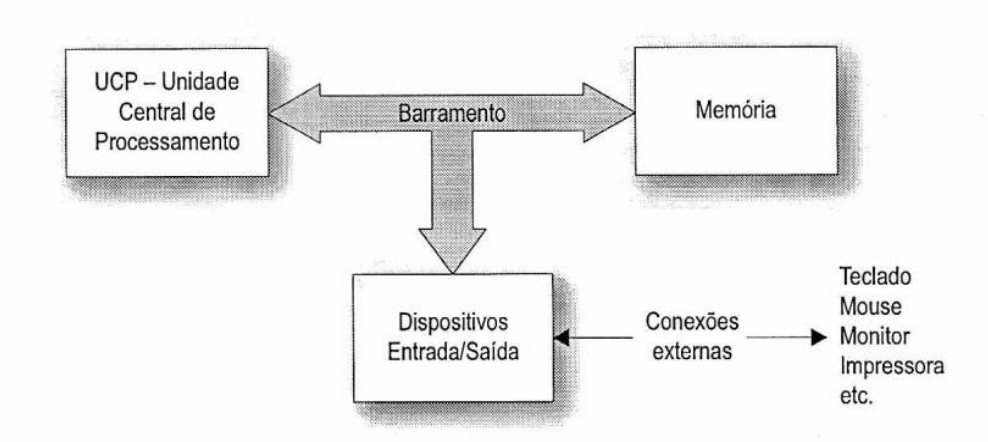
\includegraphics[width=0.5\textwidth]{figuras/Arquitetura.png}
  \end{figure}
\end{frame}


\begin{frame}{Sobre programas}
  O que é um programa?
  \begin{itemize}
    \item Uma sequência finita de instruções a serem executadas pela unidade central de processamento \cite{medina2006algoritmos}.
    \item É um algoritmo escrito em um formato compreensível pelo computador \cite{apostila2023}.
  \end{itemize}
\end{frame}

